\documentclass[fleqn, a4paper. 12pt]{ltjsarticle} % lualatex guidance.tex
\usepackage{amsmath,txfonts}
\usepackage{amssymb}
\usepackage{url}
\usepackage[margin=31mm]{geometry}
\usepackage{graphicx}
\usepackage{color}
\usepackage{appendix}
\usepackage{here}
\usepackage{float}
\newcommand{\XA}[1]{\begingroup \color{red}}
\newcommand{\AX}[1]{\endgroup}

\newcommand{\br}[1]{\left(#1\right)}                %normal brackets
\newcommand{\cbr}[1]{\left\{#1\right\}}             %curly brackets
\newcommand{\sbr}[1]{\left\lbrack #1 \right\rbrack} %square brackets

\usepackage{listings} 

\lstset{
  basicstyle={\linespread{0.6}},
  identifierstyle={\small},
  keywordstyle={\small\bfseries},
  ndkeywordstyle={\small},
  stringstyle={\small\ttfamily},
  frame={tb},
  breaklines=true,
  columns=[l]{fullflexible},
%  numbers=left,
  xrightmargin=1em,
  xleftmargin=2em,
  numberstyle={\scriptsize},
  stepnumber=1,
  numbersep=1em
}
\begin{document}
    \begin{titlepage}
      \begin{center}
      {
      \Huge 2023年度\\システムプログラミング実験}
      
      \vspace{4cm}
             {\Huge コンパイラ\\
               実験レポート\\}
             \vspace{4cm}
                    {\large 実験日:2023年12月10日(日)\\提出日:2023年12月18日(月)\\}
                    
                    {\large 学修番号:22140003\\氏名:佐倉仙汰郎}
    \end{center}  
  \end{titlepage}
  \newcommand{\fB}{f_\mathrm{B}}
  \newcommand{\fQ}{f_\mathrm{Q}}
  \newcommand{\fM}{f_\mathrm{M}}
  \newcommand{\fSTL}{f_\mathrm{STL}}
  
    \section{実験の目的}
    C言語などの高級言語のプログラムは直接CPUで実行することができない.そのため、CPUで実行できる、機械語にコンパイルする必要がある.
    本実験では、ソースコードを仮想的なスタック機械の命令コードに翻訳するコンパイラを作ることを目的とする.またそのうえで、コンパイラ作成に必要な、構文解析や字句解析について学んでいく.
    \section{開発環境}
    \begin{itemize}
      \item Central Processing Unit: 11th Gen Intel(R) Core(TM) i7-1165G7\footnote{\url{https://www.intel.co.jp/content/www/jp/ja/products/sku/208921/intel-core-i71165g7-processor-12m-cache-up-to-4-70-ghz-with-ipu/specifications.html}}, 2.80 GHz
      \item 主記憶: Double Data Rate 4 Synchronous Dynamic Random-Access Memory\footnote{\url{https://www.jedec.org/standards-documents/docs/jesd79-4a}}, 1200 MHz, 256 bit
      \item コンパイラ: gcc version 11.4.0\footnote{https://gcc.gnu.org/}
      \item コンパイルコマンド: gcc compiler.c (compiler.c はソースプログラムのファイル名である.)
      \item Operating System: Arch Linux\footnote{\url{https://archlinux.org/}} (カーネルは 5.14.8-arch1-1を使用)
  \end{itemize}

  \section{作成したプログラム}
  \begin{figure}[H]
    \centering
    \begin{lstlisting}[language=C, caption={}, label=sample-code]
      int lexan()
{
	int t;
	while(1) {
		t = getchar();
		if (t == ' ' || t == '\t')
			;
		else if ( t == '\n')
			lineno = lineno + 1;
		else if (t==':'){
		t=getchar();
		if (t=='='){
		return ASSIGN;}
		}
		else if (isdigit(t)) {
			ungetc(t, stdin);
			scanf("%d", &tokenval);    // for gcc
			//scanf_s("%d", &tokenval);    // for Visual Studio
			return NUM;
		}
		else if (isalpha(t)) {
			int p,b = 0;
			while (isalnum(t)) {
				lexbuf[b] = t;
				t = getchar();
				b = b + 1;
				if (b >= BSIZE)
					error("compiler error");
			}
			lexbuf[b] = EOS;
			if (t !=EOF)
				ungetc(t, stdin);
			p = lookup(lexbuf);
			if (p == 0)
				p = insert(lexbuf, ID);
			tokenval = p;
			return symtable[p].token;
		}
		else if (t == EOF)
			return DONE;
		else {
			tokenval = NONE;
			return t;
		}
	}
}
    \end{lstlisting}
    \caption{lexan()}
    \label{lexan}
  \end{figure}
  lexan()では、字句解析をおこなっている.標準入力を解析し正しい定数を返り値として渡すのがこの関数の目的である.
  代入演算子を読み込めるようにするために、条件文を用いて、=が読み込まれまたその次の入力が:だった場合に、新しく定義した定数ASSIGNを返している.
  また他には、数かアルファベットかなどを判断したり、行数のカウントもここで行われている.

  \begin{figure}[H]
    \centering
    \begin{lstlisting}[language=C, caption={}, label=sample-code]
      #include <stdio.h>
  
      void parse()
{
	lookahead = lexan();
	while (lookahead != DONE) {
		stmt(); match(';');
	}
}
    \end{lstlisting}
    \caption{parse()}
    \label{parse}
  \end{figure}
  parse関数では構文解析を行っている.parse関数を呼び出し字句をして常に次のトークンを確認している.stmt関数を呼び出すことで、構文解析が始まり、トークンが;だった場合に終了するようになっている.


  \begin{figure}[H]
    \centering
    \begin{lstlisting}[language=C, caption={}, label=sample-code]
      void expr()
{
	int t;
	term();
	while(1)
		switch (lookahead) {
		case '+': case '-':
			t = lookahead;
			match(lookahead); term(); emit(t, NONE);
			continue;
		default:
			return;
		}
}
    \end{lstlisting}
    \caption{expr()}
    \label{exprs}
  \end{figure}
  expr関数では、まず構文木の仕組みから次に生成されるtermを呼び出す.
  そして式として扱う加算と減算を処理する.次のトークンが+もしくは-だった場合には、さらにtermへと分岐していき、その後演算子を出力する.

  \begin{figure}[H]
    \centering
    \begin{lstlisting}[language=C, caption={}, label=sample-code]
      void stmt(){
	if(lookahead == ID){
		printf("lvalue ");
		emit(ID,tokenval);
		match(lookahead);
		if(lookahead == ASSIGN){
			match(lookahead);
			expr();
			printf(":=\n");
		}
	}
	else if(lookahead == WHILE){
		match(lookahead);
		printf("label test\n");
		cond();
		printf("go false\n");
		if(lookahead == DO){
			match(lookahead);
			stmt();
			printf("goto test\n");
			printf("label out");
		}
	}
	else if(lookahead == BEGIN){
		while(1){
			if(lookahead == END){
				break;
			}
			if(lookahead != END){
			match(lookahead);
			stmt();}
		}
	}
}
    \end{lstlisting}
    \caption{stmt()}
    \label{stmt}
  \end{figure}
  stmt関数は構文木上で文を表すために実装した関数である.stmt関数では、Identifier、ループ文、beginとendをもちいた文を処理する.
  まず次のトークンがIDだった場合、まずはそのトークンを$"lvalue ~"$として出力する.その次のトークンに進みそのトークンが代入演算子のASSIGNだった場合、expr関数を呼び出し数字を出力した後に、:=を出力する.
  トークンがWHILEだった場合、まず$"label test"$と出力し、次のトークンを読み込む.cond関数を呼び出し"go false"を出力し、条件の中身の出力が終了する.
  次のトークンがDOである場合、次のトークンに移動し、stmt関数を呼び出すことで命令内容の翻訳が完了する.最後に"goto test"と"label out"を出力し完了する.
  beginとendを用いた文では、whileループの中で、ENDが読み込まれるまで、次のトークンを読み込む$\rightarrow$stmt関数を呼び出すというサイクルを続けることで、構文木が作成される.
  ENDが読み込まれたらbreakで終了する.

  \begin{figure}[H]
    \centering
    \begin{lstlisting}[language=C, caption={}, label=sample-code]
      void term()
{
	int t;
	factor();
	while(1)
		switch (lookahead) {
		case '*': case '/': case DIV: case MOD:
			t = lookahead;
			match(lookahead); factor(); emit(t, NONE);
			continue;
		default:
			return;
		}
}
    \end{lstlisting}
    \caption{term()}
    \label{term}
  \end{figure}
  term関数ではまずfactor関数を呼び出し、構文木を作っていく.term関数の中では、乗算除算を処理するので、while文の中で、乗除算を表す演算子が読み込まれた場合、次のトークンへ移動、factor関数を呼び出す、演算子を出力という順番で処理する.
  

  \begin{figure}[H]
    \centering
    \begin{lstlisting}[language=C, caption={}, label=sample-code]
      void cond()
{
	int t;
	expr();
	while(1)
		switch (lookahead) {
		case '<':
			t = lookahead;
			match(lookahead); expr();emit(t,NONE);
			break;
		case '>':
			t = lookahead;
			match(lookahead); expr();emit(t,NONE);
			break;
			//printf(">\n");
		case '=':
			t = lookahead;
			match(lookahead); expr(); emit(t,NONE);	
			break;		//printf("=\n");
		default:
			return;
		}
}
    \end{lstlisting}
    \caption{cond()}
    \label{cond}
  \end{figure}

  cond関数では比較演算子を処理している.stmt関数でWHILE文だと判断されたときに、WHILE文の条件式にこの比較演算子は出てくるのでcond関数が呼ばれてる.
  ここではほかの関数exprなどと似たような手順を踏んでいる.次のトークンが$>,<m=$のいずれかの場合新しいトークンの呼び出し$\rightarrow$expr関数の呼び出し$\rightarrow$数値の出力を行ってる.

  \begin{figure}[H]
	\centering
	\begin{lstlisting}[language=C, caption={}, label=sample-code]
		void factor()
		{
			switch(lookahead) {
				case '(':
					match('('); expr(); match(')'); break;
				case NUM:
					printf("push ");emit(NUM, tokenval); match(NUM); break;
				case ID:
					printf("rvalue ");emit(ID, tokenval); match(ID); break;
				default:
					error("syntax error"); break;
			}
			//printf("factor finished\n");
		}
	\end{lstlisting}
	\caption{factor()}
	\label{factor}
  \end{figure}
  factor関数は構文木の葉にあたるものになる.stmt関数から呼び出され様々な形で分岐するが最終的にはこのfactor関数にたどりつく.ここでは、数、ID、括弧を処理する.
  括弧を読み込んだ時には括弧内の式を処理するためにexpr関数を呼び出しペアになる括弧をマッチさせ終了させる.数が読み込まれた場合、まず"push"を出力する.そして数をemit関数を用いて出力し、終了する.
IDを読み込まれた場合には、まず"rvalue"と出力し、その後数が読み込まれたときと同様な手順をたどる.
  その他の場合には"syntax error"となる.


  \begin{figure}[H]
	\centering
	\begin{lstlisting}[language=C, caption={}, label=sample-code]
		void match(t)
		int t;
	{
		if (lookahead == t)
			lookahead = lexan();
		else error("syntax error");
	}
	\end{lstlisting}
	\caption{match()}
	\label{match}
  \end{figure}
  match関数では、lexan関数を用いて新しいトークンを読み込む.

  \begin{figure}[H]
	\centering
	\begin{lstlisting}[language=C, caption={}, label=sample-code]
		void emit(t, tval)
		int t, tval;
	{
		switch(t) {
			case '+': case '-': case '*': case '/': case '>': case '<' : case '=':
				printf("%c\n", t); break;
			case DIV:
				printf("DIV\n"); break;
			case MOD:
				printf("MOD\n"); break;
			case NUM:
				printf("%d\n", tval); break;
			case ID:
				printf("%s\n", symtable[tval].lexptr); break;
			default:
				printf("token %d, tokenval %d\n", t, tval); break;
		}
	}
	\end{lstlisting}
	\caption{emit()}
	\label{emit}
  \end{figure}
  emit関数は、主に出力をする関数である.変更点は、比較演算子を読み込めるように、caseに追加した.
  caseを使って様々な場合において適切に出力ができるようになっている.

  \begin{figure}[H]
	\centering
	\begin{lstlisting}[language=C, caption={}, label=sample-code]
		int lookup(s)
		char s[];
	{
		int p;
		for (p = lastentry; p > 0; p = p -1)
			if (strcmp(symtable[p].lexptr, s) == 0)
				return p;
		return 0;
	}
	\end{lstlisting}
	\caption{lookup()}
	\label{lookup}
  \end{figure}
  lookup関数ではシンボルテーブル内で引数に一致するものがあるかないかを判断している.あったらpを返し、ない場合には$0$を返却する.

  \begin{figure}[H]
	\centering
	\begin{lstlisting}[language=C, caption={}, label=sample-code]
		int insert(s, tok)
		char s[];
		int tok;
	{
		int len;
		len = strlen(s);
		if (lastentry +1 >= SYMMAX)
			error("symbol table full");
		if (lastchar + len +1 >= STRMAX)
			error("lexemes array full");
		lastentry = lastentry +1;
		symtable[lastentry].token = tok;
		symtable[lastentry].lexptr = &lexemes[lastchar + 1];
		lastchar = lastchar + len + 1;
		strcpy(symtable[lastentry].lexptr, s);
		return lastentry;
	}
	\end{lstlisting}
	\caption{insert()}
	\label{insert}
  \end{figure}
  insert関数は新しいシンボルをシンボルテーブルに追加する.シンボルテーブルの容量を確認し満杯であればエラーを吐く.また、lexemes配列の容量も確認して、満杯であればこれもエラーを吐くようになっている.

  \begin{figure}[H]
	\centering
	\begin{lstlisting}[language=C, caption={}, label=sample-code]
		void init()
		{
			struct entry *p;
			for (p = keywords; p -> token; p++)
				insert(p -> lexptr, p -> token);
		}
	\end{lstlisting}
	\caption{init()}
	\label{init}
  \end{figure}
  init関数ではシンボルテーブルを初期化している.

  \begin{figure}[H]
	\centering
	\begin{lstlisting}[language=C, caption={}, label=sample-code]
		void error(m)
		char *m;
	{
		fprintf(stderr, "line %d: %s\n", lineno, m);
		exit(1);
	}
	\end{lstlisting}
	\caption{error()}
	\label{error}
  \end{figure}
  error関数はエラーメッセージを表示してプログラムを終了するためのエラー処理関数である.

  \begin{figure}[H]
	\centering
	\begin{lstlisting}[language=C, caption={}, label=sample-code]
		void main()
		{
			init();
			parse();
			exit(0);
		}
	\end{lstlisting}
	\caption{main()}
	\label{main}
  \end{figure}
  main関数ではまずシンボルテーブルを初期化して、その後字句解析を始めるここですべての入力を処理して最後に終了する.

  

  \section{プログラムの実行結果}
  \subsection{代入文}
  \begin{figure}[H]
	\centering
	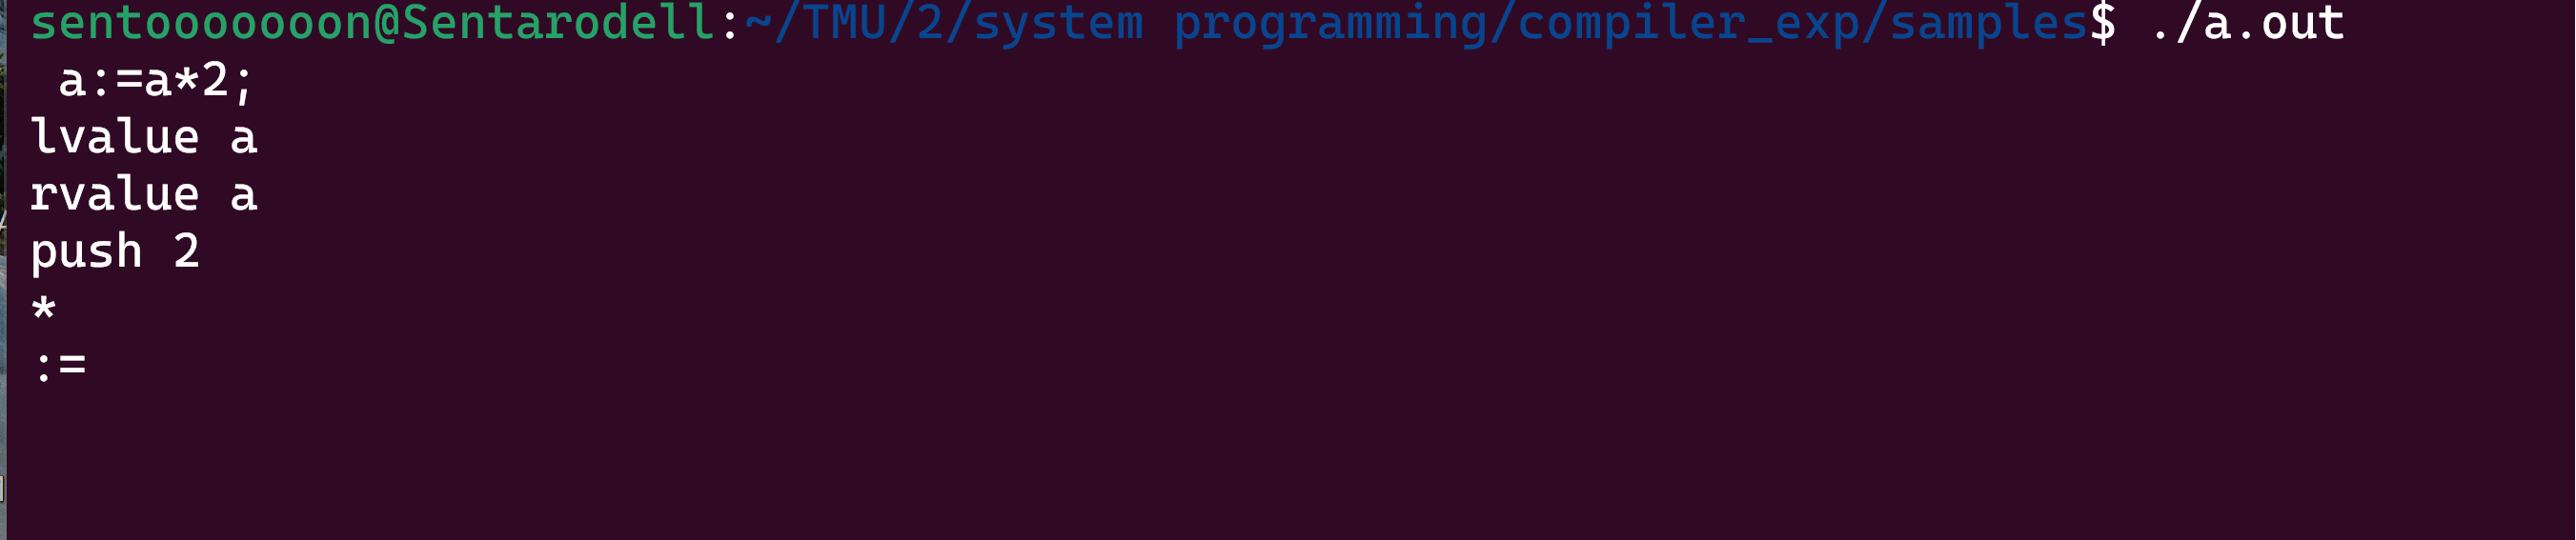
\includegraphics[width=0.8\linewidth]{"images/ASSIGN.png"}
	\caption{代入文を実行したときの結果}
	\label{fig:ASSIGN}
  \end{figure}
  
  \begin{figure}[H]
	\centering
	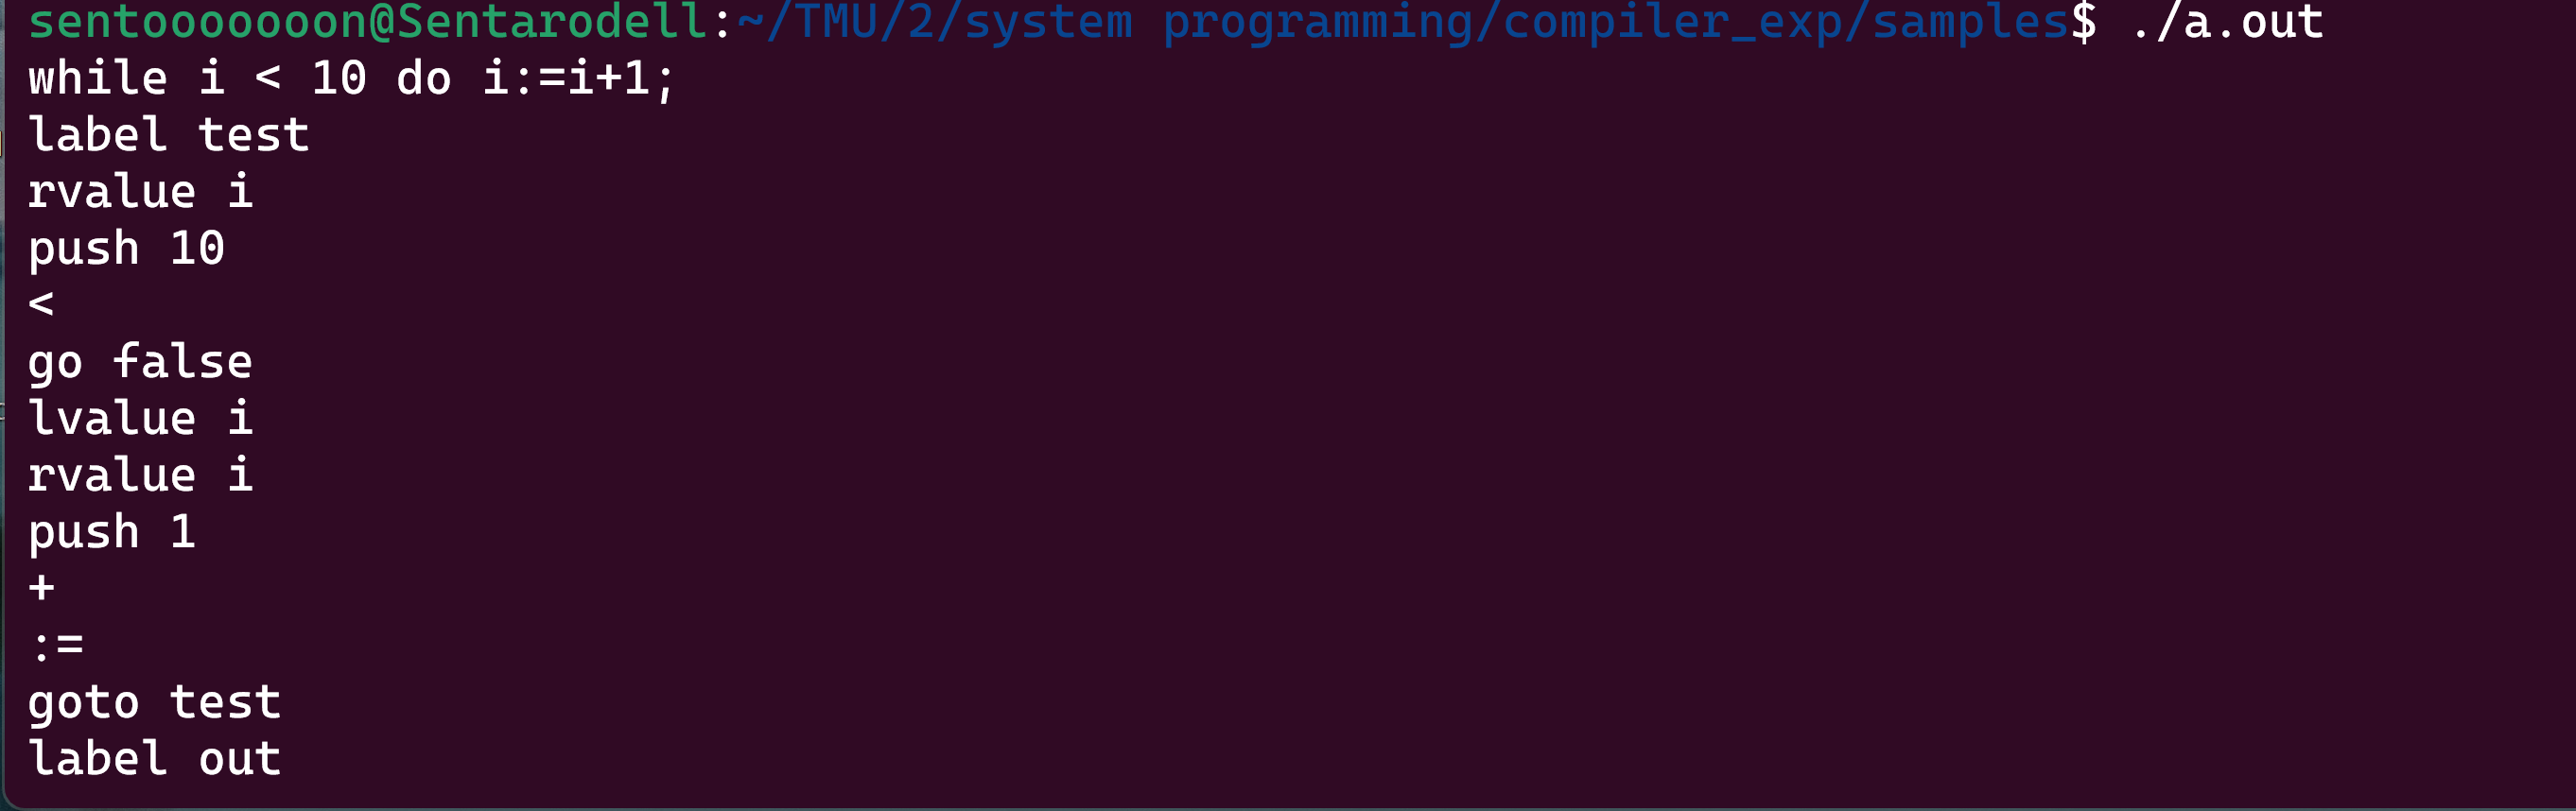
\includegraphics[width=0.8\linewidth]{"images/WHILE.png"}
	\caption{WHILE文を実行したときの結果}
	\label{fig:WHILE}
  \end{figure}

  \begin{figure}[H]
	\centering
	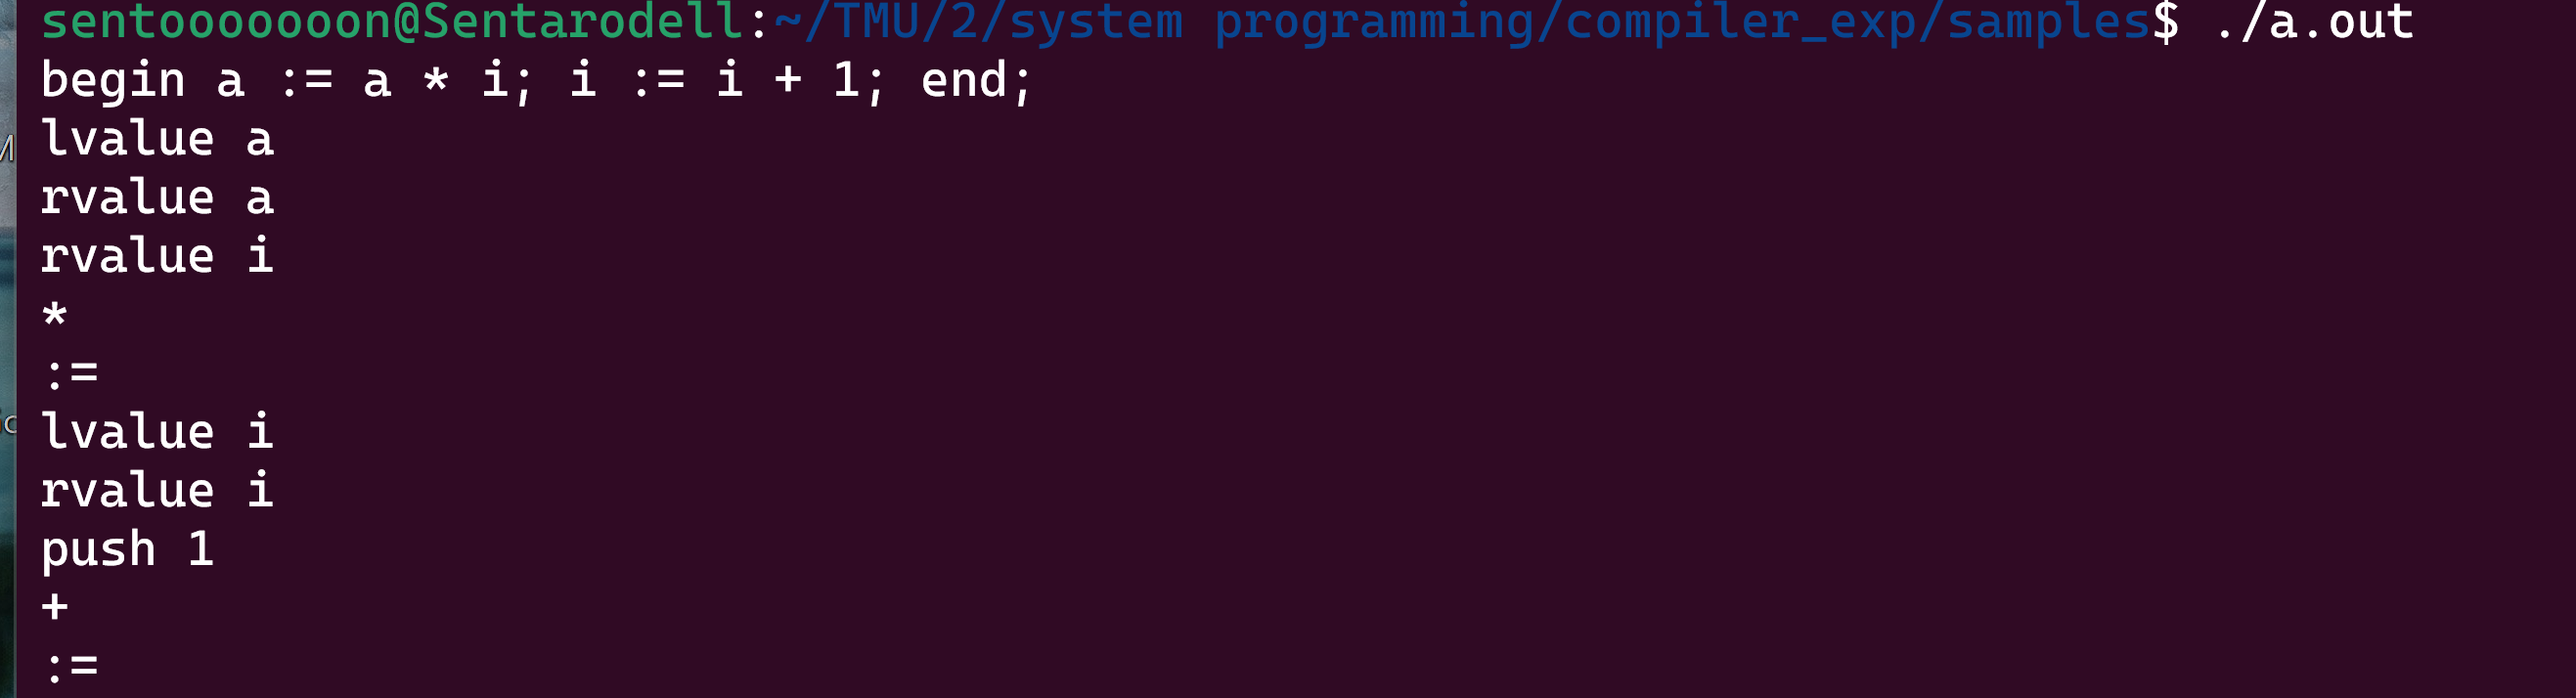
\includegraphics[width=0.8\linewidth]{"images/BEGIN.png"}
	\caption{beginを実行したときの結果}
	\label{fig:BEGIN}
  \end{figure}

  \section{まとめ}

  今回の実験は非常に私にとって大変なものであった.最初に字句解析と構文解析をテキストで理解しようと思ったがうまくいかずコードをいじりながら理解していった.
  またこのレポートを書くことでよりコンパイラの理解が深まった.
  このコンパイラ実験で関数の有用性を強く感じた.関数を分けて置くとエラーが起こった時の修正がしやすい.また構文木の再現などやれることの幅もとても広がるのだと感じた.

  \begin{appendices}
	\lstinputlisting{../samples/compiler.c}

	\end{appendices}



  
    \begin{thebibliography}{00}
        \bibitem{Sort}中田育男,コンパイラ: 作りながら学ぶ ,オーム社,2017
        \end{thebibliography}
\end{document}
